
% This LaTeX was auto-generated from an M-file by MATLAB.
% To make changes, update the M-file and republish this document.

\documentclass[11pt]{article}
\usepackage{amsmath,amsfonts,amsthm,amssymb}
\usepackage{fullpage,fancyhdr}
\usepackage[pdftex]{graphicx}
\usepackage[usenames,dvipsnames]{color}
\usepackage{listings}
\usepackage{courier}
\usepackage{ifthen}
\usepackage{setspace}
\usepackage{lastpage}
\usepackage{colortbl}
\usepackage{extramarks}
\usepackage{chngpage}
\usepackage{soul}
\usepackage{graphicx,float,wrapfig}
\usepackage{epstopdf}
\usepackage{geometry}
\usepackage{pdfcolmk}
\usepackage{hyperref}
\DeclareGraphicsRule{.tif}{png}{.png}{`convert #1 `dirname #1`/`basename #1 .tif`.png}

\definecolor{lightgray}{gray}{0.5}
\definecolor{darkgray}{gray}{0.3}
\definecolor{MyDarkGreen}{rgb}{0.0,0.4,0.0}

\topmargin=-0.45in      %
\evensidemargin=0in     %
\oddsidemargin=0in      %
\textwidth=6.5in        %
\textheight=9.0in       %
\headsep=0.25in         %
\headheight = 14pt

\pagestyle{fancyplain}

% For faster processing, load Matlab syntax for listings
\lstloadlanguages{Matlab}%
\lstset{language=Matlab,
        frame=single,
        basicstyle=\ttfamily,
        keywordstyle=[1]\color{Blue}\bf,
        keywordstyle=[2]\color{Purple},
        keywordstyle=[3]\color{Blue}\underbar,
        identifierstyle=,
        commentstyle=\usefont{T1}{pcr}{m}{sl}\color{MyDarkGreen}\small,
        stringstyle=\color{Purple},
        showstringspaces=false,
        tabsize=5,
        % Put standard MATLAB functions not included in the default
        % language here
        morekeywords={xlim,ylim,var,alpha,factorial,poissrnd,normpdf,normcdf},
        % Put MATLAB function parameters here
        morekeywords=[2]{on, off, interp},
        % Put user defined functions here
        morekeywords=[3]{likelihood,nfoldconv,statistics},
        morecomment=[l][\color{Blue}]{...},
        numbers=left,
        firstnumber=1,
        numberstyle=\tiny\color{Blue},
        stepnumber=5
        }

 
\fancyhf{}
 
\lhead{\fancyplain{}{Michael Carroll}}
\chead{\fancyplain{}{MECH7710}}
\rhead{\fancyplain{}{\today}}
\rfoot{\fancyplain{}{\thepage\ of \pageref{LastPage}}}

\sloppy
\setlength{\parindent}{0pt}



\title{MECH7710 - HW1\\
{\large \begin{par}
Random Variables and Probability
\end{par} \vspace{1em}
}}
\author{Michael J. Carroll}


\begin{document}
\maketitle
\section*{Problem 1}
\subsection*{Part A - 6 dice numbered 1,2,3,4,5,6}
    
\begin{lstlisting}[language=matlab]
pdf_matrix = 1/6 * ones(6,6);
pdf_combined = nfoldconv(pdf_matrix);
[mean,variance] = statistics(pdf_combined);
true_norm = normpdf([1:length(pdf_combined)],mean,sqrt(variance));
if plots,
    createfigure(true_norm, pdf_combined, 'Problem 1 - Part A')
end
\end{lstlisting}
{\color{lightgray} \small\begin{verbatim}
mean =
   21.0000
variance =
   17.5000
\end{verbatim}}
\begin{figure}[here]
	\begin{center}
		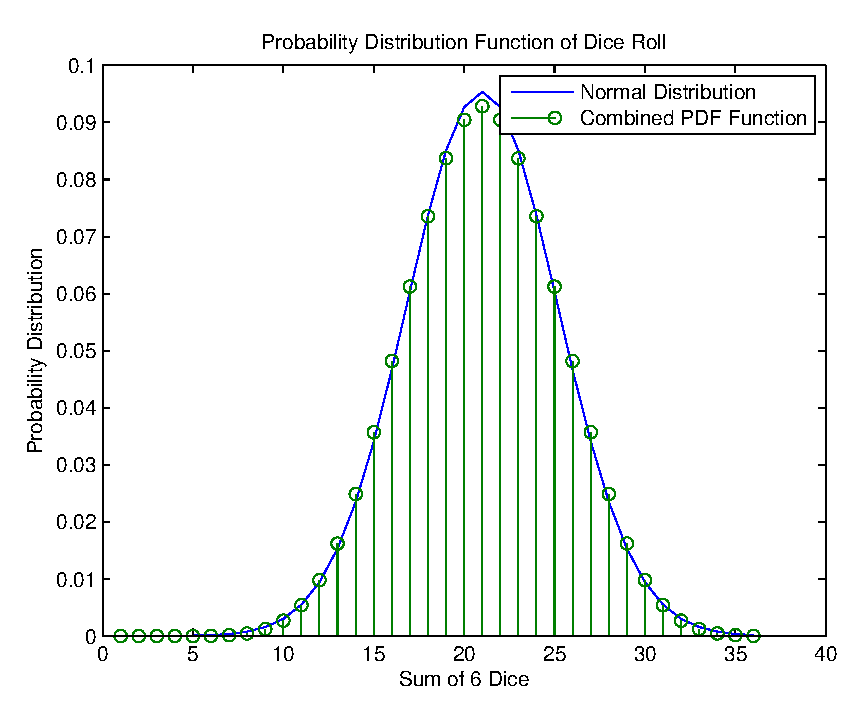
\includegraphics [width=3.2in]{hw1_01.eps}
		\caption{PDF of a Dice Roll - Problem 1A}
		\label{fig:pr1-a}
	\end{center}
\end{figure}

\subsection*{Part B - 6 dice numbered 4,5,6,7,8,9}
\begin{lstlisting}[language=matlab]
pdf_matrix = 1/6 * [zeros(6,3),ones(6,6)];
pdf_combined = nfoldconv(pdf_matrix);
[mean,variance] = statistics(pdf_combined);
true_norm = normpdf([1:length(pdf_combined)],mean,sqrt(variance));
if plots,
    createfigure(true_norm, pdf_combined, 'Problem 1 - Part B')
end
\end{lstlisting}
{\color{lightgray} \small\begin{verbatim}
mean =
   39.0000
variance =
   17.5000
\end{verbatim}}
\begin{figure}[htb]
	\begin{center}
		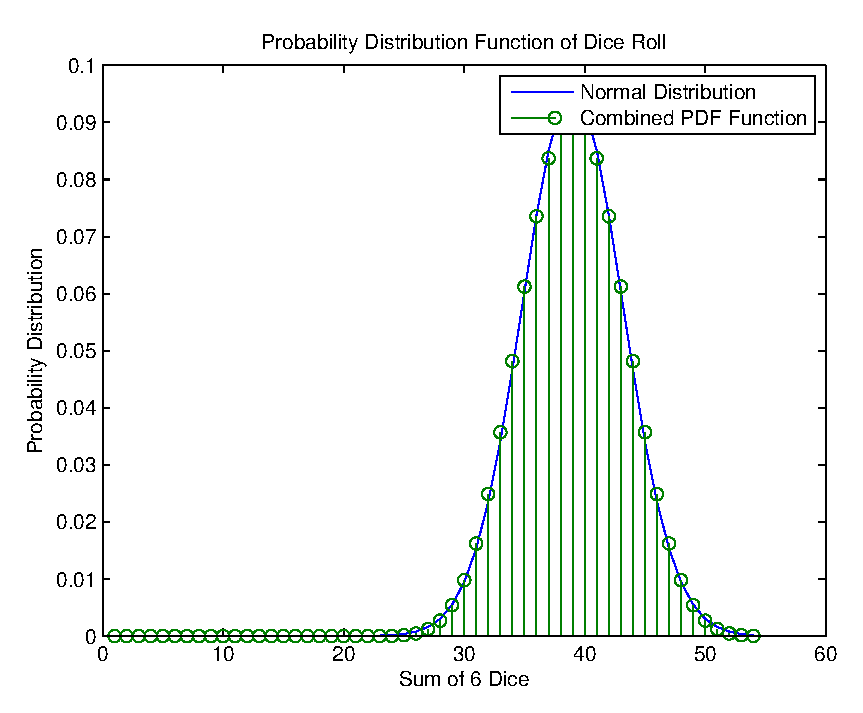
\includegraphics [width=4in]{hw1_02.eps}
		\caption{PDF of a Dice Roll - Problem 1B}
		\label{fig:pr1-b}
	\end{center}
\end{figure}

\newpage
\subsection*{Part C - 6 dice numbered 1,1,3,3,3,5}
\begin{lstlisting}[language=matlab]
pdf_matrix = [...
    1/3 * ones(6,1), zeros(6,1), ...
    1/2 * ones(6,1), zeros(6,1), ...
    1/6 * ones(6,1), zeros(6,1)];
pdf_combined = nfoldconv(pdf_matrix);
[mean,variance] = statistics(pdf_combined);
true_norm = normpdf([1:length(pdf_combined)],mean,sqrt(variance));
if plots,
    createfigure(true_norm, pdf_combined, 'Problem 1 - Part C')
end
\end{lstlisting}
{\color{lightgray} \small\begin{verbatim}
mean =
    16
variance =
   11.3333
\end{verbatim}}
\begin{figure}[htb]
	\begin{center}
		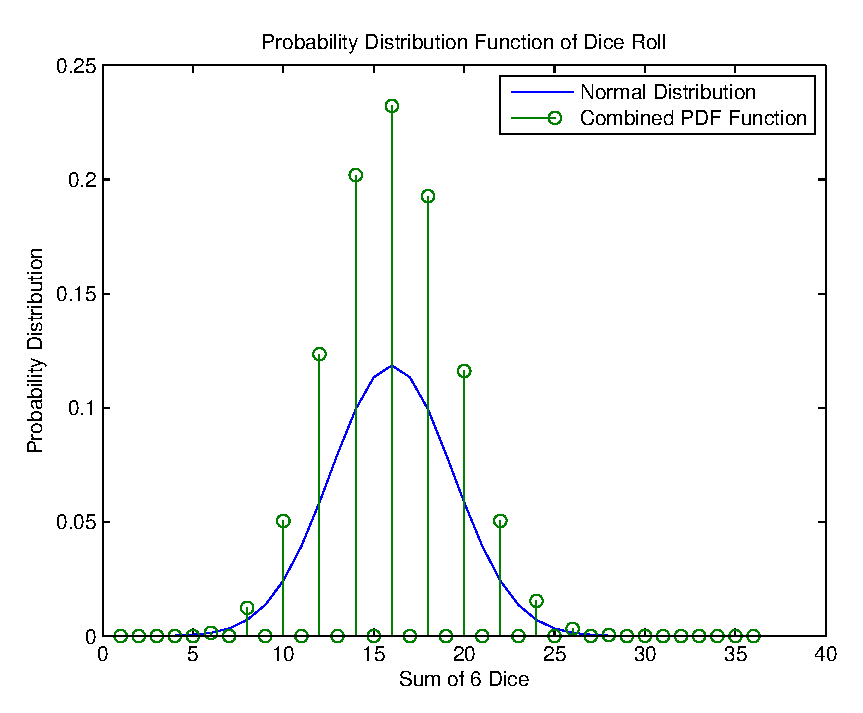
\includegraphics [width=4in]{hw1_03.eps}
		\caption{PDF of a Dice Roll - Problem 1C}
		\label{fig:pr1-c}
	\end{center}
\end{figure}

\newpage
\subsection*{Part D - 3 dice numbered 1,2,3,4,5,6 and 3 numbered 1,1,3,3,3,5}
\begin{lstlisting}[language=matlab]
pdf_matrix = [...
    1/6*ones(3,6); ...
    1/3 * ones(3,1), zeros(3,1), ...
    1/2 * ones(3,1), zeros(3,1), ...
    1/6 * ones(3,1), 1/6*zeros(3,1)];

pdf_combined = nfoldconv(pdf_matrix);
[mean,variance] = statistics(pdf_combined);
true_norm = normpdf([1:length(pdf_combined)],mean,sqrt(variance));
if plots,
    createfigure(true_norm, pdf_combined, 'Problem 1 - Part D')
end
\end{lstlisting}
{\color{lightgray} \small\begin{verbatim}
mean =
   18.5000
variance =
   14.4167
\end{verbatim}}
\begin{figure}[htbp]
	\begin{center}
		\includegraphics [width=4in]{hw1_04.eps}
		\caption{PDF of a Dice Roll - Problem 1D}
		\label{fig:pr1-d}
	\end{center}
\end{figure}

\clearpage

\section*{Problem 2}
\subsection*{Part A - Mean, Central Moment, Mean Squared, Variance and Covariance}

\begin{lstlisting}[language=matlab]
pdf_die_1 = 1/6 * ones(1,6);
pdf_die_2 = 1/6 * ones(1,6);

die = 1:6;
joint_pdf = pdf_die_1' * pdf_die_2;

[mean_1, variance_1, c_moment_1, mean_sq_1] = statistics(pdf_die_1);
\end{lstlisting}

{\color{lightgray} \small\begin{verbatim}
mean_v1 =
    3.5000

variance_v1 =
    2.9167

c_moment_v1 =
     0

mean_sq_v1 =
   15.1667
\end{verbatim}}

\subsection*{Part B - Covariance Matrix}
\begin{lstlisting}[language=matlab]
% Covariance of 2 independant variables is 0.
covariance = sum(sum((die-mean_1)'*(die-mean_1) * joint_pdf));

P = [variance_1, covariance; covariance, variance_1]
\end{lstlisting}

{\color{lightgray} \small\begin{verbatim}
covariance =
     0
P =
    2.9167         0
         0    2.9167
\end{verbatim}}

\newpage
\subsection*{Part C, D, E, and F}
\begin{par}
Find the PDF matrix for the variables $v_1=x_1$ and $v_2 = x_1 + x_2$. Use [1:6, 1:12], with the first column zeros.
\end{par}

\begin{lstlisting}[language=matlab]
v_1 = [1:6]; v_2 = [1:12];

joint_pdf = zeros(6,12); joint_v = zeros(6,12);

for ii=1:6,
    joint_pdf(ii,ii+[1:6]) = 1/36;
    for jj=1:6,
        joint_v(ii,ii+jj) = ii+jj;
    end
end

[mean_v1, variance_v1, c_moment_v1, mean_sq_v1] = statistics(pdf_die_1)

mean_v2 = sum(sum(joint_v .* joint_pdf));
mean_sq_v2 = sum(sum(joint_v.^2 .* joint_pdf));
c_moment_v2 = sum(sum((joint_v - mean_v2) .* joint_pdf));
variance_v2 = sum(sum((joint_v - mean_v2).^2 .* joint_pdf));

covariance_12 = sum(sum((v_1 - mean_v1)'*(v_2 - mean_v2).*joint_pdf));

P = [variance_v1, covariance_12;
    covariance_12, variance_v2]
rho_12 = covariance_12/(sqrt(P(1,1)) * sqrt(P(2,2)))
\end{lstlisting}

{\color{lightgray} \small\begin{verbatim}
mean_v2 =
    7.0000
mean_sq_v2 =
   54.8333
c_moment_v2 =
   1.9151e-15
variance_v2 =
    5.8333
covariance_12 =
    2.9167
P =
    2.9167    2.9167
    2.9167    5.8333
rho_12 =
    0.7071
\end{verbatim}}
           
\newpage

\section*{Problem 3}
\begin{par}
Two random vectors are called uncorrelated if $P = 0$
\end{par} \vspace{1em}

\subsection*{Part A}
\begin{par}
 Show that independent random vectors are uncorrelated.
\end{par}
\begin{align}
 P(x_1,x_2) &= E\{(x_1 - \bar{x_1})(x_2 - \bar{x_2})^T\} = 0 \\
  &= E[x_1 x_2 - \bar{x_1}x_2 - x_1\bar{x_2} + \bar{x_1}\bar{x_2} \\
  &= E[x_1 x_2] - E[\bar{x_1}x_2] - E[x_1\bar{x_2}] + E[\bar{x_1}\bar{x_2}] \\
  &= E[x_1 x_2] - \bar{x_1}\bar{x_2} - \bar{x_1}\bar{x_2} + \bar{x_1}\bar{x_2} \\
  &= E[x_1 x_2] - \bar{x_1}\bar{x_2} \\
  &= \iint{x_1 x_2 p(x_1,x_2) dx_1 dx_2} - \bar{x_1}\bar{x_2} \\
  &= \int{x_1 p(x_1)dx_1}\int{x_2 p(x_2)dx_2} - \bar{x_1}\bar{x_2}\\
  &=  \bar{x_1}\bar{x_2} - \bar{x_1}\bar{x_2} = 0
\end{align}

\subsection*{Part B}
\begin{par}
 Show that uncorrelated Gaussian random vectors are independent.
\end{par}

\begin{align}
P(x_1,x_2) &= \frac{1}{2\pi\sigma_1 \sigma_2 \sqrt{1-\rho^2}} 
\exp{\left(\frac{-1}{2(1-\rho^2)} \left[\frac{(x_1 - \bar{x_1})^2}{\sigma_1^2} + \frac{(x_2 - \bar{x_2})^2}{\sigma_2^2} - \frac{2\rho(x_1 - \bar{x_1}) (x_2 - \bar{x_2})}{\sigma_1\sigma_2} \right]\right)}
\end{align}

Uncorrelated implies that $\rho = 0$, reducing this to:

\begin{align}
P(x_1,x_2) &= \frac{1}{2\pi\sigma_1 \sigma_2} 
\exp{\left(\frac{-1}{2} \left[\frac{(x_1 - \bar{x_1})^2}{\sigma_1^2} + \frac{(x_2 - \bar{x_2})^2}{\sigma_2^2}\right]\right)} \\
&= \frac{1}{\sqrt{2\pi}\sigma_1} \exp{\left(\frac{-(x_1 - \bar{x_1})^2}{2\sigma_1^2}\right)}
\frac{1}{\sqrt{2\pi}\sigma_2} \exp{\left(\frac{-(x_2 - \bar{x_2})^2}{2\sigma_2^2}\right)}\\
P(x_1,x_2) &= P(x_1)P(x_2)
\end{align}

The joint probability distribution function reduces to two single-variable probability distribution functions, which are independent from each other.

\newpage
\section*{Problem 4}
Consider a sequence created by throwing a pair of dice and summing the numbers which are $\{-2.5, -1.5, -0.5, 0.5, 1.5, 2.5\}$.
    
\begin{lstlisting}[language=matlab]
v_0 = [-2.5, -1.5, -0.5, 0.5, 1.5, 2.5];
pdf_0 = 1/6 * ones(1,6);
pdf_new = conv(pdf_0,pdf_0);
v_new = [-5:5];
mean_v0 = sum(pdf_new .* v_new)
variance_v0 = sum((v_new - mean_v0).^2 .* pdf_new)
\end{lstlisting}
   {\color{lightgray} \small\begin{verbatim}
mean_v0 =
    0
variance_v0 =
    5.8333
\end{verbatim} }

If we generate a new random sequence as: $V_N(k+1) = (1-r)V_N(k) + rV_o(k)$

The mean in steady state can be determined by writing the $V_N$ formula as an infinite sum.

$$ \mu_{Vn} = \sum_{-\infty}^{\infty} r(1-r)^n V_o[n] * PDF(V_o[n]) = E[V_o] * \sum_{0}^{\infty} r(1-r)^n = 0$$

Likewise, the variance can be calculated easily due to the mean of zero.  It is simply squaring the previous term.

$$ \sigma_n^2 = \sum_{-\infty}^{\infty} r^2 (1-r)^{2n} V_o[n]^2 * PDF(V_o[n]) = \sigma_o^2 * \sum_{0}^{\infty} r^2 (1-r)^n = \frac{r}{r-2} \sigma_o^2$$

I then used Laplace transforms to determine the autocorrelation function of the random sequence:

$$\frac{V_N(s)}{V_o(s)} = \frac{r}{s+(r-1)} = r \exp{\left[(r-1)*|\tau|\right]} $$

The covariance function follows from the autocorrelation function:

$$ R_v(k)= r \exp{\left[(r-1)*|L|\right]} $$


The practical constraints on r is that it may not exceed 2.0 and it should not go under 0.0.  Going outside these two bounds will cause the random signal to exponentially grow,
which will sacrifice BIBO stability.  There is no other reasonable analysis that we could do on the system if it was determined to be unstable.


\newpage
\section*{Problem 5}
\begin{par}
Given a random variable \textbf{x}, determine the mean and variance.

The mean can be determined with the definition.  The integral will only be 
evaluated between 0 and 2, where the PDF is not equal to zero.
\end{par} \vspace{1em}

\[PDF(x) = \begin{cases}
 0 & x < 0 \\
 x/2 & 0 \leq x < 2 \\
 0 & x \geq 2
\end{cases}\]

\begin{align}
 \bar{x} &= \int_{-\infty}^{\infty}{x \cdot PDF(x) dx} \\
 \bar{x} &= \int_{0}^{2}{x \cdot x/2 dx} \\
 \bar{x} &= \frac{x^3}{6} \Bigr| _{0}^{2} \\
 \bar{x} &= 4/3
\end{align}

\begin{par}
 Similarly, the variance may be found using the definition.
\end{par}

\begin{align}
 \sigma_x^2 &= \int_{-\infty}^{\infty}{(x - \bar{x})^2 \cdot PDF(x) dx} \\
 \sigma_x^2 &= \int_{0}^{2}{(x-4/3)^2 \cdot x/2 dx} \\
 \sigma_x^2 &= \int_{0}^{2}{(1/2 x^3 - 4/3 x^2 + 8/9 x) dx} \\
 \sigma_x^2 &= 2 - 32/9 + 16/9 \\
 \sigma_x^2 &= 2/9
\end{align}


\newpage   
\section*{Problem 6}
\begin{par}
 Consider a normally distributed two-dimensional vector x, with mean value zero and
$$P_x = \left[\begin{matrix}
 2 & 1 \\
 1 & 4 \end{matrix}\right]$$
\end{par}

\begin{lstlisting}[language=matlab]
P_x = [2, 1; 1, 4];

Mu = [0;0];
[V,D] = eig(P_x);

likelihood(Mu,P_x,[0.25, 1.0, 1.5]);
\end{lstlisting}

The eigenvalues of this matrix are found using the eig command in MATLAB.

{\color{lightgray} \small\begin{verbatim}
D =
    1.5858         0
         0    4.4142
\end{verbatim} }

The principle axes in the case of this matrix would be along the eigenvectors.  This can also be found using the eig command in MATLAB.
{\color{lightgray} \small\begin{verbatim}
V =
   -0.9239    0.3827
    0.3827    0.9239
\end{verbatim} }

\begin{figure}[here]
	\begin{center}
		\includegraphics [width=4in]{hw1_05.eps}
		\caption{Likelihood Ellipses for $c = {0.25, 1.0, 1.5}$}
		\label{fig:}
	\end{center}
\end{figure}

\begin{center}
\begin{tabular}{l|l|l|l}
C & 0.25 & 1.0 & 1.5\\
\hline
Table Value & 0.5987 & 0.8413 & 0.9332\\
Likelihood & 19.74\% & 68.26\% & 86.64\%
\end{tabular}
\end{center}

        
\section*{Problem 7}
\begin{par}
If $x \sim N(0,\sigma_x^2)$ and $y= 2x^2$, then:
\end{par}

\begin{align}
 p_x[y] &= p_x[f^{-1}(y)]\left|\frac{\delta f^{-1}(y)}{\delta y} \right| \\
x &= (y/2)^{1/2} \\
\left|\frac{\delta f^{-1}(y)}{\delta y} \right| &= \frac{1}{2 \sqrt{2y}} \\
p_x[y] &= \frac{1}{2 \sqrt{2y}} \left(f_x\left(\frac{y}{2}\right)^{1/2} - f_x\left(\frac{y}{2}\right)^{1/2}\right) \\
p_x[y] &= \frac{1}{\sigma_x \sqrt{4\pi y}} \exp\left[\frac{-y}{4 \sigma_x^2}\right]  & y \geq 0 \\
       &= 0 & y < 0
\end{align}

\begin{par}
 The new probability distribution function is zero up to the origin, then infinite at the origin, and declines as y approaches positive infinity.  
This is due to the idea that this new PDF is similar to distribution of power, with the most probable power being 0.  The variable y is no longer a normal random variable.
\end{par}


\begin{lstlisting}[language=matlab]
X = linspace(0,5,1000);
sigma = 2;
fx_pdf = normpdf(linspace(-5,5,1000),0,sigma);
fy_pdf = 1./(sigma * sqrt(4*pi*X)) .* exp(-X./(4*sigma^2));
plot(X,fy_pdf)
hold
plot(linspace(-5,5,1000),fx_pdf)
\end{lstlisting}

\begin{figure}[here]
	\begin{center}
		\includegraphics [width=3.2in]{hw1_06.eps}
		\caption{Normal PDF vs. PDF of y}
		\label{fig:pr6-1}
	\end{center}
\end{figure}


\clearpage
\section*{Appendix A - Calculate Statistics of a Vector}
\lstinputlisting{../statistics.m}

\section*{Appendix B - Perform N-fold Convolution}
\lstinputlisting{../nfoldconv.m}    

\newpage
\section*{Appendix C - Draw Likelihood Ellipses}
\lstinputlisting{../likelihood.m}    


\end{document}

